\subsection{Data description}
We have a two-class classification problem. The training data $Xtrain$ contains 1500 observations, each 32 dimensional. One training sample has 31 real valued features and 1 categorical feature, the 14th feature. Our task is to predict the category for unseen test data, consisting in 1500 samples. We measure the accuracy of our estimation using $RMSE$, $0-1 loss$ and $log-loss$. 

\subsection{Data visualization and cleaning}
We noticed the samples were not equally distributed among classes, about $35\%$ of the samples were coming from one class and $65\%$ from the other. We did not have time to study the implications of this on our model estimation. We changed the labeling from -1/1 to 0/1 because our cost function was better expressed using 0 and 1.

The training data was again not centered as seen in $Fig.$\ref{fig:dist_classification}
 After changing feature 14 to a dummy variable we normalized the data to have 0 mean and std 1.We noticed more outliers in the data of classification than in the one from regression. We removed outliers the same way as in the regression task which left us with 1431 samples (4$\%$ of the data).
\begin{figure}[h]
  \begin{subfigure}[b]{0.5\textwidth}
   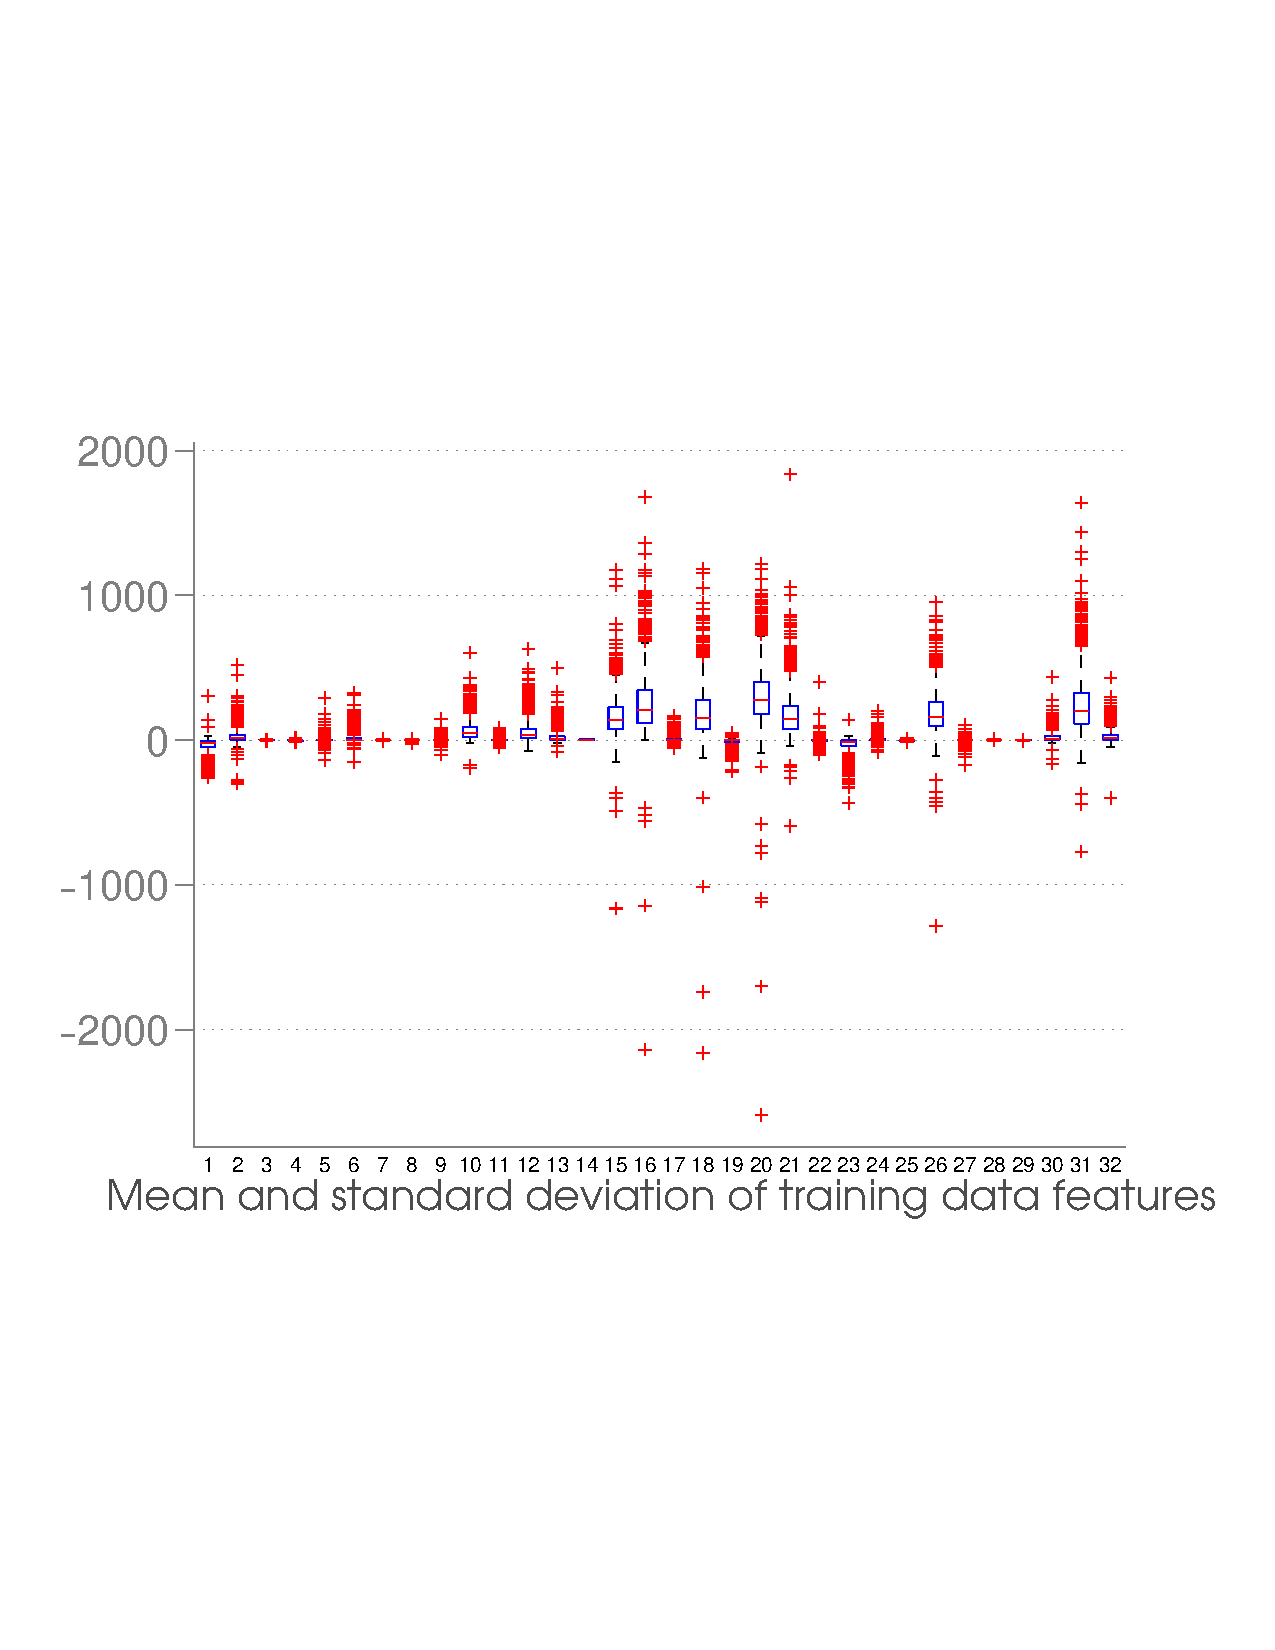
\includegraphics[width=\textwidth]{figures/classification_distribution.pdf}
    \caption{Mean and standard deviation for the training data features. The input is not normalised and contains outliers.}
    \label{fig:dist_classification}
  \end{subfigure}
  \caption{• Data visualization. }
\end{figure}

\subsection{Logistic Regression}

We applied Logistic Regression (logRegression) and Penalized Logistic Regression (penLogRegression) using gradient descent with learning rate $\alpha$. Best results are obtained on the train accuracy of $97.14\%$ with $\alpha = 10$. We obtained the optimal $\alpha$ for logRegression   and penalty factor $\lambda$ for penLogisticRegression using the cross validation technique with a $50\%-50\%$ split for training and validation data.

In penLogRegression, the choice of penalty factor ($\lambda$) is crucial.  We sampled 400 values for $\lambda$s in the interval  $10^{-2}$ to $10^3$. As can be seen in Figure \ref{fig:Lambda_pLr}, for small $\lambda$ values, training error is much lower than the test error while for large $\lambda$ values the test error gets as high as the training error which is a sign of under-fitting. 

For small $\lambda$ values, the training and test error estimated in penLogisticRegression show very similar behavior with the ones for logRegression. The same $\alpha$ value that is obtained for logRegression  also gives the best accuracy for penLogisticRegression.

\begin{figure}[h]
  \begin{subfigure}[b]{0.5\textwidth}
   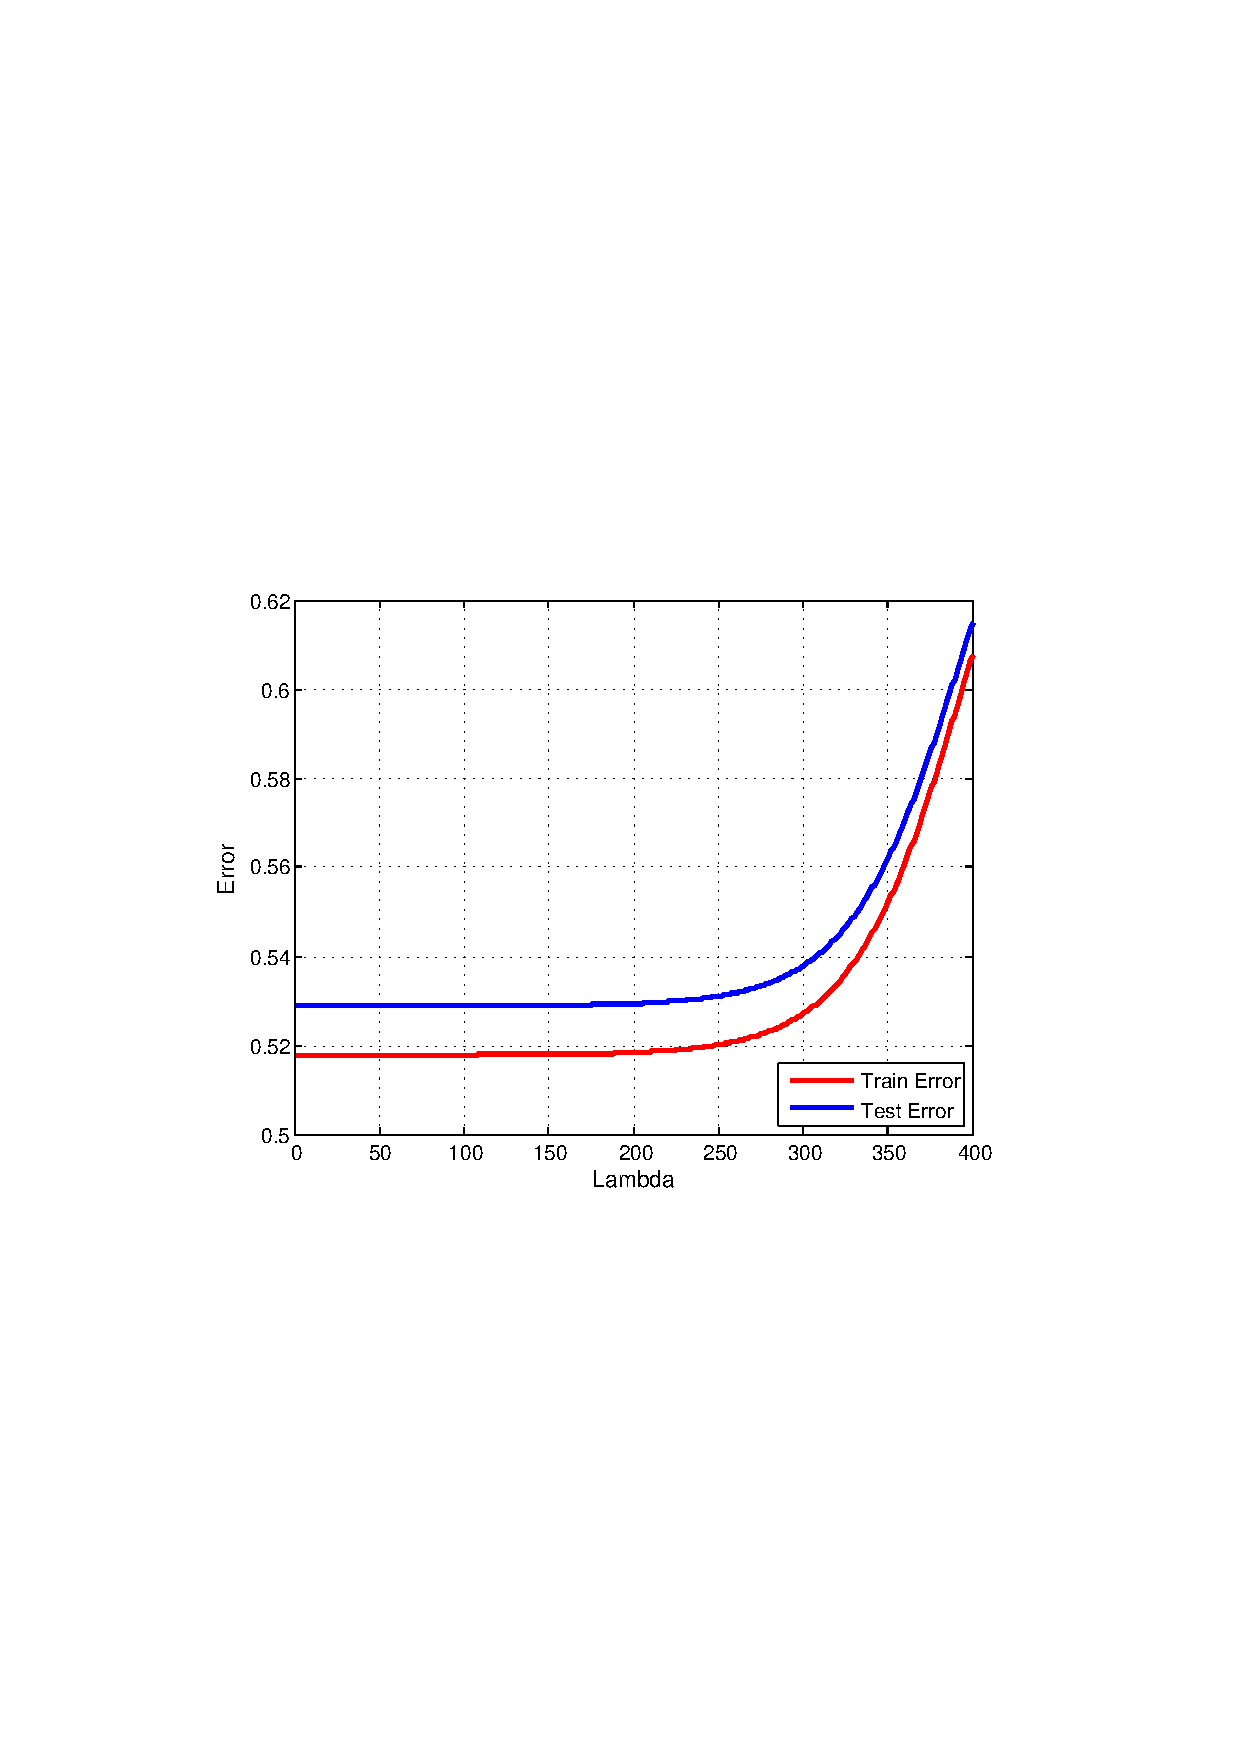
\includegraphics[clip, trim=4cm 9cm 3cm 10cm, width=\textwidth]{figures/Lambda_pLG.pdf}
    \caption{Train and test error assessment with penalty factor ($\lambda$) for penalized logistic regression
    for 50-50 split.}
    \label{fig:Lambda_pLr}
  \end{subfigure}
  \hfill
  \begin{subfigure}[b]{0.45\textwidth}
    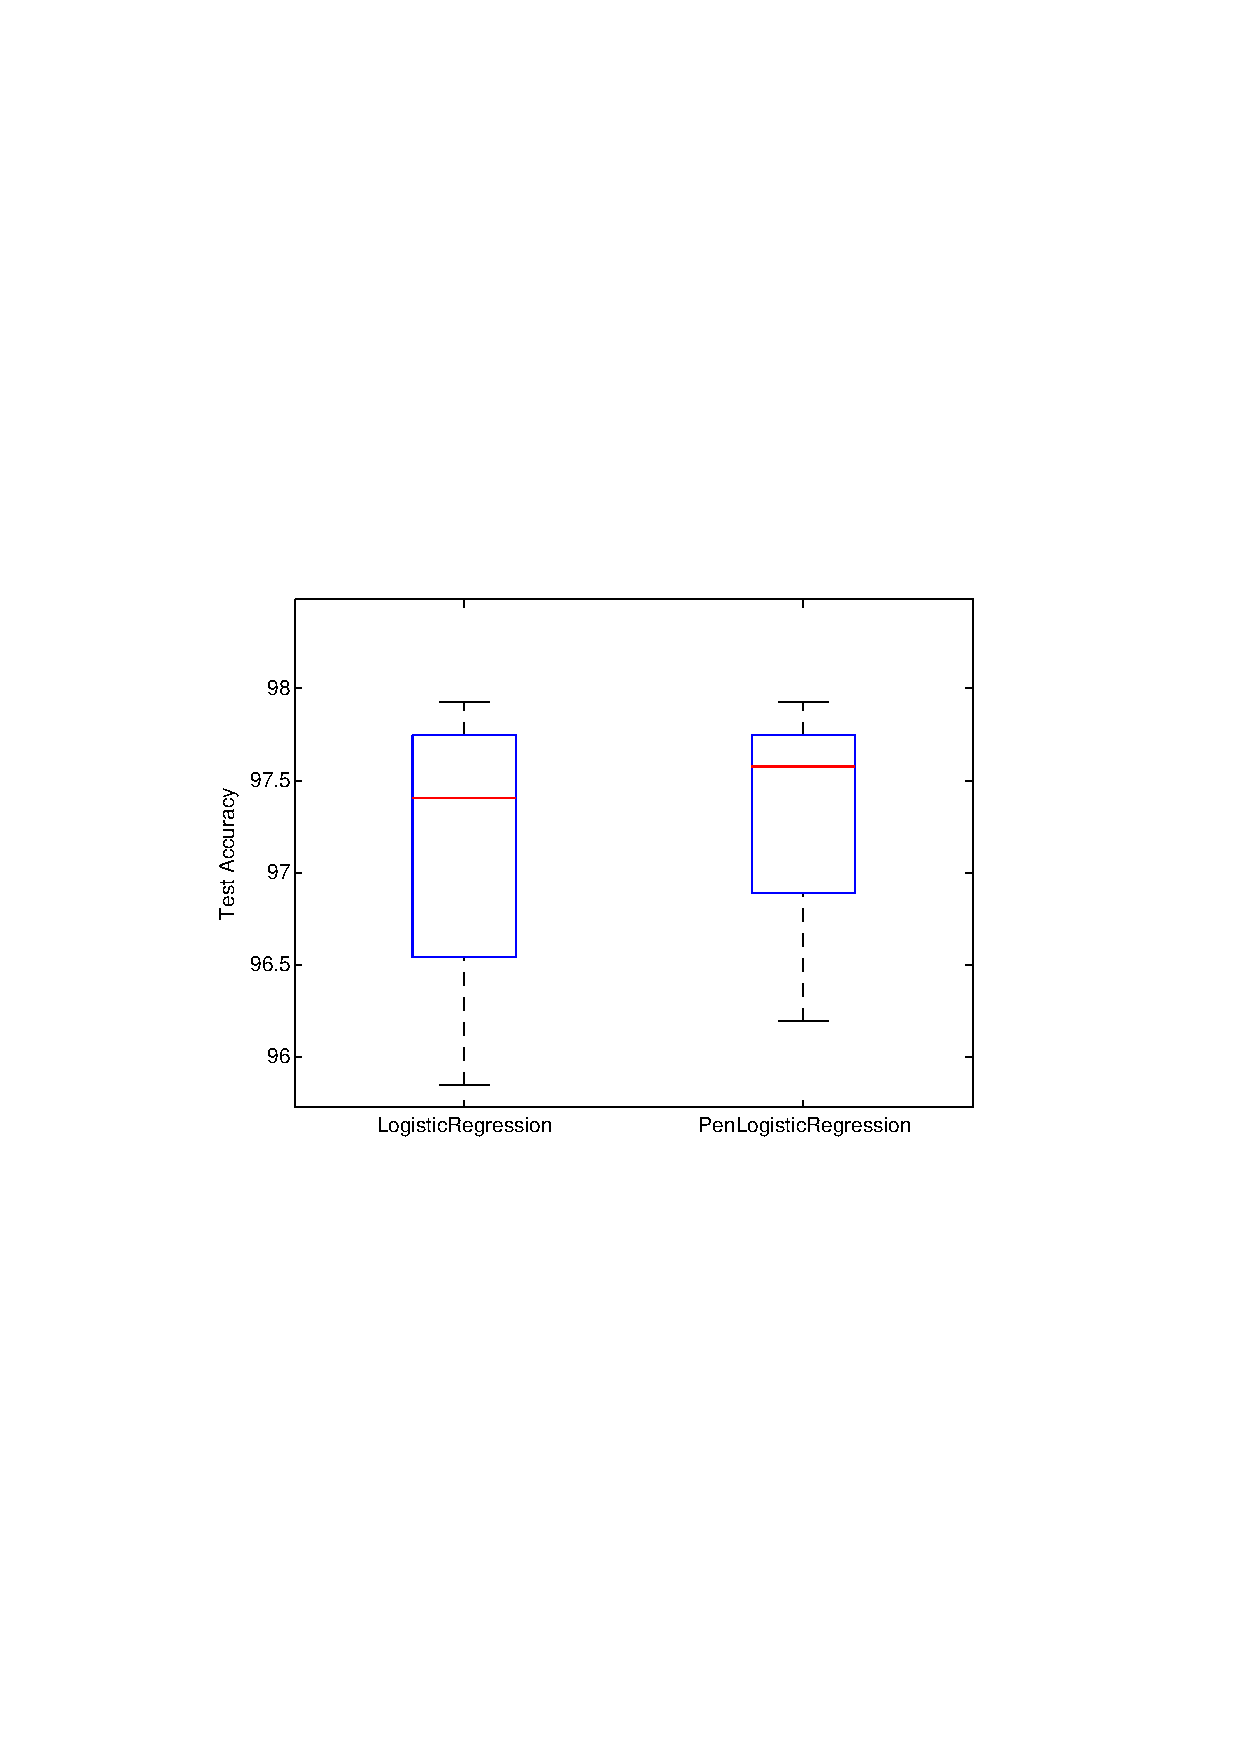
\includegraphics[clip, trim=4cm 10cm 3cm 10cm, width=\textwidth]{figures/comparison_LR_pLR.pdf}
    \caption{Comparison of logistic regression and penalized logistic regression based on validation accuracy}
    \label{fig:comp_LR_pLR}
  \end{subfigure}
\end{figure}


\ref{fig:comp_LR_pLR} shows the classification accuracy percentage  of logRegression and penLogRegression on the test data (4-fold cross validation). The improvements with penLogRegression is little but significant.  
Best results are obtained on the test accuracy of $97.318\%$ with $\lambda=0.5$ and ($\alpha=1$).

\begin{table}[h!]
\begin{center}
    \begin{tabular}{ | l | l | l | p{5cm} |}
    \hline
    Method & RMSE & 0-1-Loss & Log-Loss \\ \hline
    Logistic Regression & 0.147896 & 0.020743 & 105.151844 \\ \hline
    Pen Logistic Regression & 0.122288 & 0.014693 & 75.380959 \\ \hline
    \end{tabular}
\end{center}
\caption{Some prediction error estimates for the test data}
\label{table:test_errors}
\end{table}
 
The table \ref{table:test_errors} shows error measurements of the test data with $\alpha=10.0$ and $\lambda=1.0$ using $RMSE$, $0-1 loss$ and $log-loss$. Increasing the value of $alpha$ decreases all error estimations until a maximum $alpha=10.0$ value which gives the best prediction accuracy.

\subsection{Feature transformation}
We experimented with polynomial, exponential, sqrt(abs*)) of the values
but did not manage to improve the previous results obtained using penalized logistic regression. Our best model setup (alpha = lambda = degree =) had a recognition rate of approx 96$\%$, when we used a polynomial of degree 2.
Since the model worked  and but not better just as it is
and since simpler models are preferred, we considered this not to be so relevant.